% body_v2.tex — Paper body with HIGH-severity fixes H1, H2, H4 applied
% Original: main.tex (v1, 29 pages)
% Changes: see v1_to_v2_diff.tex for detailed changelog

% --- Abstract ----------------------------------------------------------------
\begin{abstract}
\noindent
Volatility targeting (VT) strategies are often characterized as repackaged trend following, since VT alpha is largely absorbed by a time-series momentum (TSMOM) factor. We show that this characterization conflates statistical alpha absorption with economic value. The primary benefit of VT is not alpha generation but drawdown insurance: across 22 assets spanning equities, commodities, bonds, and international markets, VT's maximum drawdown (MDD) protection is preserved after TSMOM removal (5-asset K1192 canonical point estimates: SPY 103.7\%, 50/50 SPY/GLD 95.6\%, DIA 106.2\%, QQQ 109.0\%, IWM 102.2\%), while the Sharpe ratio channel is only partially attributable to trend following. A 252-day moving-block bootstrap delivers 90\% CI lower bounds of 76--93\% across the five-asset canonical table (K1376); a stationary-bootstrap robustness check with 3--5 year expected block lengths yields lower bounds of 90--100\% (K1417), \emph{strengthening} the non-erosion conclusion under longer-memory resampling. Point estimates above 100\% should be interpreted cautiously: they indicate that hedging does not damage the drawdown channel, but part of the incremental improvement can arise mechanically when the hedge trims exposure during momentum-crash rebound windows. The mechanism is therefore best described as VIX-level-based position sizing that remains distinct from return-direction momentum in net economic effect. Cross-sectionally, the GJR-GARCH leverage effect parameter ($\gamma$) predicts VT's TSMOM loading ($r = 0.564$, $p = 0.006$, $N = 22$), providing an empirical regularity consistent with the leverage effect channel driving VT--TSMOM overlap, though this cross-sectional link ($N = 22$) operates only across asset classes, not within equity sectors ($r = 0.163$, NS, $N = 11$). A split-sample robustness check---estimating $\gamma$ from 2007--2016 and TSMOM loading from 2017--2026---yields $r = 0.793$ ($p < 0.001$, K1193 canonical), though part of this strengthening likely reflects asset-class composition and safe-haven loading shifts in the later subsample rather than cleaner causal identification. Internationally, US VIX serves as a broad de-risking signal: 13 of 13 equity markets achieve significant MDD improvement (K1178 canonical: average 24.9 percentage points, $t = 10.25$), with VIX sensitivity predicting the magnitude of protection ($r = -0.806$, $p < 0.001$, Spearman $\rho = -0.835$). A direct test confirms that five canonical trend-following strategies (SMA, Faber, Golden Cross, Dual Momentum, MA+VT) all fail the \citet{harvey2016} $t > 3.0$ threshold when applied to SPY, while VT's MDD protection remains robust across sub-periods. These results reframe VT as drawdown insurance whose net protection survives TSMOM removal, overturning earlier interpretations of VT as repackaged trend following.

\medskip
\noindent
\textbf{Keywords:} volatility targeting, time-series momentum, leverage effect, drawdown, VIX, cross-asset

\medskip
\noindent
\textbf{JEL Classification:} C22, G11, G12, G15
\end{abstract}

\newpage

% =============================================================================
% 1. INTRODUCTION
% =============================================================================
\section{Introduction}

Volatility targeting (VT) and time-series momentum (TSMOM) are two of the most extensively documented phenomena in empirical asset pricing. VT strategies, which scale portfolio exposure inversely with forecasted volatility, have been shown to improve risk-adjusted returns across equity factors \citep{moreira2017}, multiple asset classes \citep{harvey2018}, and individual country markets \citep{lai2026a}. TSMOM strategies, which take long (short) positions in assets with positive (negative) past returns, generate significant abnormal returns across 58 futures markets \citep{moskowitz2012}, with evidence extending to century-long samples across diverse asset classes \citep{hurst2017}. Despite their apparent differences in construction, a growing literature suggests these two strategies may share a common source of returns. \citet{cederburg2020} challenge VT on utility grounds, arguing that the strategy does not improve investor welfare after accounting for higher moments---a critique we revisit through the lens of drawdown protection.

The connection between VT and trend following emerges from the leverage effect \citep{black1976, christie1982}. When equity prices decline, volatility typically rises, causing VT to mechanically reduce exposure---effectively deleveraging after losses, much like a trend-following strategy. This mechanical channel is well-documented: \citet{barroso2015} show that volatility-scaling momentum strategies eliminates momentum crashes, precisely because the leverage effect creates a natural hedge that scales down exposure when volatility spikes after losses. \citet{hood2025} provide direct evidence that approximately 91\% of equity VT alpha is absorbed by a TSMOM factor when applied to 50 futures contracts. This raises a fundamental question: \textit{Is VIX-based de-risking simply trend following by another name?}

We argue the answer is no. While VT and TSMOM share a common channel through the leverage effect, VT possesses a distinct economic mechanism that trend following does not replicate. Specifically, we decompose VT's benefits into two channels: (i)~a \textit{Sharpe ratio channel} that operates partially through implicit TSMOM exposure, and (ii)~a \textit{maximum drawdown (MDD) channel} that operates through VIX-level-based position sizing and is largely orthogonal to trend following in net outcome. This dual-mechanism framework resolves the tension between the statistical finding that TSMOM absorbs VT alpha and the practical observation that VT provides economically meaningful drawdown insurance even when alpha is not statistically significant. Our results also address the \citet{cederburg2020} critique: even if VT does not generate significant alpha, the preservation of MDD protection after TSMOM removal (K1192 canonical point estimates 95.6--109.0\% across five US equity assets, with block bootstrap 90\% CI lower bounds at 76--93\%) constitutes an economically distinct benefit that utility-based tests may underweight, especially for investors who value drawdown protection in the spirit of habit or surplus-consumption preferences \citep{campbell1999}.

Our paper makes three contributions. First, we show that the leverage effect parameter from GJR-GARCH estimation ($\gamma$) predicts VT's TSMOM loading cross-sectionally across 22 assets ($r = 0.564$, $p = 0.006$), an empirical regularity consistent with the leverage effect channel through which VIX-based de-risking mimics trend following. We emphasize that this cross-sectional association ($N = 22$, mixed asset classes) establishes a statistical link rather than a causal mechanism. A potential endogeneity concern arises because both $\gamma$ and the TSMOM loading are estimated from the same return series: a split-sample robustness check (estimating $\gamma$ from 2007--2016 and TSMOM loading from 2017--2026) yields $r = 0.793$ ($p < 0.001$, K1193 canonical), but we interpret the increase conservatively because it partly reflects a 2017--2026 regime shift in which international and safe-haven loadings flipped from near-zero to positive. This link holds across asset classes (equities vs.\ commodities vs.\ bonds) but breaks down within equity sectors ($r = 0.163$, NS, $N = 11$), where gamma variation is insufficient to differentiate TSMOM exposure. This boundary condition is new to the literature.

Second, we decompose VT's benefits into Sharpe and MDD components using TSMOM-hedged portfolio construction. After removing TSMOM exposure, MDD protection is preserved across five assets (K1192 canonical point estimates: SPY 103.7\%, 50/50 SPY/GLD 95.6\%, DIA 106.2\%, QQQ 109.0\%, IWM 102.2\%), while the Sharpe ratio improvement is only modestly reduced. Block bootstrap inference (10,000 replications, block size = 252 days) confirms that MDD retention is statistically robust: the 90\% confidence intervals (fraction definition) are [93\%, 182\%] for SPY, [76\%, 190\%] for 50/50, [82\%, 154\%] for DIA, [89\%, 210\%] for QQQ, and [87\%, 184\%] for IWM, with lower bounds at 76--93\%. A stationary-bootstrap re-check with longer expected block lengths leaves this non-erosion conclusion unchanged (K1417 task audit). We treat $>100\%$ estimates as evidence that hedging does not damage the drawdown channel, not as proof of a separate dominant mechanism, because some enhancement can arise when the hedge reduces exposure during rebound phases of momentum crashes \citep{daniel2016}. The TSMOM contribution to Sharpe improvement is small (the K898 back-calculated estimate is approximately 5.3\% of total strategy Sharpe, subject to ongoing forensic reconciliation against the originally reported 1.4\% figure), while the alpha reduction reflects compositional reallocation rather than value destruction. This demonstrates that VT's primary economic value---drawdown insurance---operates through a channel distinct from trend following.

Third, we present broad evidence that US VIX serves as a de-risking signal for global equity markets. Across 13 international equity ETFs (7 developed, 6 emerging), all 13 achieve MDD improvement under a simple 12/VIX overlay (K1178 canonical: average 24.9 percentage points, $t = 10.25$), while only 2 of 13 show Sharpe improvement. VIX sensitivity predicts the magnitude of MDD protection ($r = -0.806$, $p < 0.001$, Spearman $\rho = -0.835$), consistent with an ``insurance pricing'' relationship: investors pay approximately $4\%$/year Sharpe drag for broad drawdown protection. We interpret this pricing channel cautiously: VIX likely bundles expected volatility, variance risk premium, and downside-protection demand rather than isolating a single structural primitive \citep{bollerslev2009, bondarenko2019}. This international pattern is consistent with the global financial cycle documented by \citet{miranda2020}, in which US financial conditions propagate to international markets through capital flows and risk appetite.

Our paper contributes to several literatures. We extend \citet{hood2025} by decomposing the dual channel (Sharpe vs.\ MDD), which their framework does not distinguish. We clarify that while VT embeds asset-specific TSMOM exposure through the leverage effect, this is distinct from diversified managed-futures strategies that trade across dozens of uncorrelated markets \citep{moskowitz2012, baltas2013}. Our finding that VT's embedded momentum exposure operates through the leverage effect channel complements \citet{daniel2016}, who show that momentum crashes are driven by precisely this leverage-effect-induced volatility clustering. We also extend the ``volatility-as-insurance'' perspective of \citet{lai2026a} to a global setting, building on the foundational work of \citet{fleming2001}, who established the economic value of volatility timing in a portfolio context.

The remainder of the paper is organized as follows. Section~2 describes our data and methodology. Section~3 presents the empirical results. Section~4 discusses implications and limitations. Section~5 concludes.


% =============================================================================
% 2. DATA AND METHODOLOGY
% =============================================================================
\section{Data and Methodology}

\subsection{Data}

We employ three asset samples. The \textit{primary sample} comprises 22 assets across equities (SPY, QQQ, IWM, XLF, XLE, DIA, EEM, EFA, FXI, EWZ, EWJ, EWG, EWU, EWA, INDA), commodities (GLD, SLV, USO), bonds (TLT, LQD, HYG), and real estate (VNQ). Daily return data span January 2005 to March 2026, sourced from Yahoo Finance.

The \textit{international sample} consists of 13 country-level equity ETFs: 7~developed markets (EFA, EWJ, EWG, EWU, EWA, EWC, VGK) and 6~emerging markets (EEM, FXI, EWZ, INDA, EWT, MCHI). The \textit{sector sample} comprises 11 SPDR sector ETFs (XLB, XLE, XLF, XLI, XLK, XLP, XLU, XLV, XLY, XLRE, XLC) with data from December 1998 to March 2026.

VIX data are obtained from the CBOE. The risk-free rate is the daily 13-week Treasury bill rate (IRX), time-varying throughout the sample. Fama--French five-factor data (MKT, SMB, HML, RMW, CMA), the momentum factor (MOM), and the betting-against-beta factor (BAB) are obtained from Kenneth French's data library and AQR, respectively.

\subsection{Volatility Targeting Construction}

We implement VIX-based VT following \citet{bozovic2024}:
\begin{equation}
w_t = \min\!\left(\frac{12}{\text{VIX}_t}, 1.0\right),
\label{eq:vt_weight}
\end{equation}
where $w_t$ denotes the fraction of the portfolio allocated to the risky asset, with the remainder in cash (proxied by SHY). To avoid look-ahead bias, we use \textit{lagged weights}: VIX at the end of month $t$ determines the allocation for month $t+1$. Rebalancing is monthly, with transaction costs of 10 basis points per round trip. The threshold of 12 follows \citet{lai2026a}, who show that any target in $[6, 20]$ produces qualitatively similar results.

\subsection{TSMOM Factor Construction}

Following \citet{moskowitz2012}, we construct a time-series momentum factor using the sign of the past 252-day (12-month) return:
\begin{equation}
\text{TSMOM}_t = \text{sign}(r_{t-252:t}) \times r_t,
\label{eq:tsmom}
\end{equation}
where $r_{t-252:t}$ is the cumulative return over the past 252 trading days.

To address correlated-regressor bias, we construct an \textit{orthogonalized} TSMOM factor by projecting TSMOM onto the market factor:
\begin{equation}
\text{TSMOM}_t^{\perp} = \text{TSMOM}_t - \hat{\beta}_{\text{MKT}} \cdot \text{MKT}_t,
\label{eq:tsmom_orth}
\end{equation}
where $\hat{\beta}_{\text{MKT}}$ is estimated from a full-sample regression. This ensures that the TSMOM loading in subsequent regressions captures momentum exposure beyond what is already explained by the market factor \citep{hood2025}.

\subsection{Alpha Decomposition}

We estimate a sequence of nested models to decompose VT alpha:
\begin{align}
\text{M1:} \quad r_{\text{VT},t} - r_{f,t} &= \alpha_1 + \beta_1 \, \text{MKT}_t + \varepsilon_t, \label{eq:m1} \\
\text{M2:} \quad r_{\text{VT},t} - r_{f,t} &= \alpha_2 + \beta_1 \, \text{MKT}_t + \beta_2 \, \text{TSMOM}_t^{\perp} + \varepsilon_t, \label{eq:m2} \\
\text{M3:} \quad r_{\text{VT},t} - r_{f,t} &= \alpha_3 + \beta_1 \, \text{MKT}_t + \beta_2 \, \text{TSMOM}_t^{\perp} + \boldsymbol{\beta}_{\text{FF}} \cdot \mathbf{F}_t + \varepsilon_t, \label{eq:m3}
\end{align}
where $\mathbf{F}_t$ includes SMB, HML, RMW, CMA, MOM, and BAB. All standard errors are Newey--West HAC \citep{newey1987} with automatic lag selection: $\ell = \lfloor 4(T/100)^{2/9} \rfloor$ \citep{newey1994}.

Alpha reduction from model $k$ to model $k+1$ is defined as:
\begin{equation}
\Delta\alpha_{k \to k+1} = \frac{\alpha_k - \alpha_{k+1}}{\alpha_k} \times 100\%.
\label{eq:alpha_reduction}
\end{equation}

\subsection{Pure VT Alpha Construction}

To isolate VT's residual alpha after removing trend-following exposure, we construct a TSMOM-hedged portfolio:
\begin{equation}
r_{\text{PureVT},t} = r_{\text{VT},t} - \hat{\beta}_{\text{TSMOM},t} \cdot \text{TSMOM}_t,
\label{eq:pure_vt}
\end{equation}
where $\hat{\beta}_{\text{TSMOM},t}$ is estimated from a rolling 252-day regression using only data from the preceding 252 trading days $[t-252, t-1]$; no information from period $t$ or later enters the weight computation at time $t$. The lagged VIX weight (Eq.~\ref{eq:vt_weight}) and the lagged TSMOM hedge are applied simultaneously, ensuring the TSMOM-hedged portfolio is fully implementable without look-ahead bias. We compare the Sharpe ratio and MDD of VT, PureVT, and a standalone TSMOM strategy.

\subsection{Cross-Sectional Tests}

We test whether the leverage effect predicts VT's TSMOM exposure. For each asset $i$, we estimate the GJR-GARCH(1,1) model \citep{glosten1993}:
\begin{equation}
\sigma_{i,t}^2 = \omega_i + (\alpha_i + \gamma_i \cdot \mathbb{1}_{r_{i,t-1}<0}) \, r_{i,t-1}^2 + \beta_i \, \sigma_{i,t-1}^2,
\label{eq:gjr}
\end{equation}
where $\gamma_i$ captures the asymmetric volatility response. We then compute Pearson and Spearman correlations between $\gamma_i$ and the TSMOM loading $\hat{\beta}_{\text{TSMOM},i}^{\perp}$ across assets, with bootstrap 95\% confidence intervals (5,000 replications).

\subsection{MDD Retention Bootstrap Inference}

To provide statistical inference for MDD retention---a single extreme-value statistic with high sampling variability---we employ a block bootstrap procedure. We apply this procedure to all 22 assets in our primary sample plus the 50/50 SPY/GLD composite, extending K1192's five-asset canonical estimates. For each asset, we:

\begin{enumerate}
\item Draw 10,000 block bootstrap samples from the daily return series, using a block size of 252 trading days (one year) as the baseline resampling scheme for drawdown dynamics.
\item For each bootstrap sample, recompute: (a) the buy-and-hold MDD, (b) the VT MDD, and (c) the TSMOM-hedged VT MDD.
\item Compute the MDD retention rate for each bootstrap sample as:
\begin{equation}
\text{MDD Retention}_b = \frac{\text{MDD}_{\text{B\&H},b} - \text{MDD}_{\text{Hedged VT},b}}{\text{MDD}_{\text{B\&H},b} - \text{MDD}_{\text{VT},b}},
\label{eq:mdd_retention_boot}
\end{equation}
where $b$ indexes the bootstrap replication.
\item Report the 5th and 95th percentiles of the bootstrap distribution as the 90\% confidence interval.
\end{enumerate}

This moving-block bootstrap approach accounts for the serial dependence in daily returns and the path-dependent nature of maximum drawdown, providing baseline inference for an extreme-value statistic that standard asymptotic theory does not easily cover. Because drawdown dependence can extend beyond a single calendar year, we also check the main inference with a stationary bootstrap using multi-year expected block lengths (K1417 task audit); that longer-memory resampling does not materially weaken the qualitative conclusion that the drawdown channel survives TSMOM hedging.


% =============================================================================
% 3. EMPIRICAL RESULTS
% =============================================================================
\section{Empirical Results}

\subsection{VT Has Significant TSMOM Exposure}

Table~\ref{tab:alpha_decomp} reports the alpha decomposition for all 22 assets. Under the CAPM-only specification (M1), VT generates positive alpha for 14 of 22 assets, though only SPY and DIA approach conventional significance levels with Newey--West $t$-statistics above 1.4. The average annualized alpha across all assets is $-0.27\%$, reflecting the ``insurance premium'' of VT \citep{lai2026a}.

Adding the orthogonalized TSMOM factor (M2) reveals substantial trend-following exposure. Of the 22 assets, 17 exhibit statistically significant TSMOM loadings ($|t| > 1.96$), with all equity assets showing positive loadings (mean $\hat{\beta}_{\text{TSMOM}}^{\perp} = 0.087$ for equities). The TSMOM loading is economically meaningful: for SPY, $\hat{\beta}_{\text{TSMOM}}^{\perp} = 0.121$ ($t = 7.65$), implying that a one-standard-deviation increase in the TSMOM factor raises VT returns by approximately 12.1 basis points per day.

Non-equity assets display qualitatively different TSMOM loadings. Gold (GLD) and real estate (VNQ) show \textit{negative} TSMOM loadings ($-0.073$ and $-0.094$, respectively), consistent with their inverted or near-zero leverage effects. TLT shows a marginally negative loading ($-0.078$, $t = -4.55$), reflecting bonds' tendency to rally (fall) when equities fall (rise) during risk-off (risk-on) episodes.

The $\Delta\alpha$ column reports the percentage of M1 alpha absorbed by adding orthogonalized TSMOM. For assets with positive M1 alpha, the absorption ranges from near-zero (EWJ: 0.3\%) to substantial (DIA: 54.0\%, EFA: 54.6\%), reflecting cross-asset variation in embedded trend-following exposure. The orthogonalization ensures that TSMOM$^{\perp}$ captures momentum exposure \textit{beyond} the market factor, so these alpha reductions reflect genuine trend-following content rather than MKT re-attribution. The $R^2$ improvement from adding TSMOM is substantial for equity assets (e.g., SPY: $0.802 \to 0.867$, $\Delta R^2 = 0.065$) but modest for non-equity assets (GLD: $0.864 \to 0.874$, $\Delta R^2 = 0.010$).

The TSMOM loading is robust to the choice of VIX threshold in the VT formula. Re-estimating M2 for SPY across all integer thresholds from 8 to 20, the orthogonalized TSMOM coefficient remains highly significant throughout ($t$-statistics ranging from 7.98 to 10.91, all $p < 0.001$, K79).\footnote{K79 refers to the paper-folder robustness sweep \texttt{paper/vt-trend-following/experiments/paper3\_fixes.json}; cf.~\texttt{experiments.md} for the full mapping. The sweep covers integer VIX thresholds 8--20 and reports both raw and orthogonalized TSMOM loadings.} The point estimate varies modestly ($\hat{\beta}_{\text{TSMOM}}^{\perp} \in [0.10, 0.14]$), confirming that the embedded trend-following exposure is a structural feature of VIX-based de-risking rather than an artifact of a particular calibration choice.


% --- Table 1: Alpha Decomposition ---
\begin{table}[H]
\centering
\begin{threeparttable}
\caption{VT Alpha Decomposition: CAPM vs.\ CAPM + TSMOM (N = 22)}
\label{tab:alpha_decomp}
\small
\begin{tabular}{@{}lcccccccc@{}}
\toprule
& & \multicolumn{3}{c}{M1: CAPM Only} & \multicolumn{3}{c}{M2: CAPM + TSMOM$^{\perp}$} & \\
\cmidrule(lr){3-5} \cmidrule(lr){6-8}
Asset & $\gamma$ & $\alpha$ (\%) & $t_{\text{NW}}$ & $R^2$ & $\beta_{\text{TSMOM}}^{\perp}$ & $t_{\text{NW}}$ & $R^2$ & $\Delta\alpha$ (\%) \\
\midrule
\multicolumn{9}{@{}l}{\textit{Panel A: Equity Assets}} \\
SPY   & 0.261 & 1.35  & 1.44 & 0.802 & 0.121 & 7.65$^{***}$ & 0.867 & 26.9 \\
QQQ   & 0.225 & 1.55  & 1.44 & 0.830 & 0.112 & 6.58$^{***}$ & 0.871 & 27.3 \\
DIA   & 0.235 & 1.19  & 1.24 & 0.788 & 0.148 & 11.57$^{***}$ & 0.886 & 54.0 \\
IWM   & 0.144 & $-$0.19 & $-$0.16 & 0.816 & 0.137 & 9.96$^{***}$ & 0.885 & -- \\
XLF   & 0.174 & 1.35  & 1.03 & 0.807 & 0.142 & 11.58$^{***}$ & 0.885 & 45.7 \\
XLE   & 0.078 & $-$1.31 & $-$0.88 & 0.809 & 0.113 & 6.95$^{***}$ & 0.856 & -- \\
EEM   & 0.121 & $-$2.80 & $-$2.09 & 0.774 & 0.142 & 8.56$^{***}$ & 0.849 & -- \\
EFA   & 0.152 & $-$0.77 & $-$0.77 & 0.801 & 0.125 & 8.11$^{***}$ & 0.861 & 54.6 \\
FXI   & 0.069 & $-$2.96 & $-$1.89 & 0.805 & 0.131 & 7.68$^{***}$ & 0.862 & 19.6 \\
EWZ   & 0.074 & $-$3.69 & $-$1.91 & 0.797 & 0.121 & 6.05$^{***}$ & 0.839 & 35.6 \\
EWJ   & 0.101 & $-$2.27 & $-$1.25 & 0.504 & $-$0.006 & $-$0.62 & 0.504 & 0.3 \\
EWG   & 0.117 & $-$4.81 & $-$2.40 & 0.593 & 0.020 & 1.76$^{*}$ & 0.593 & $-$0.4 \\
EWU   & 0.135 & $-$3.85 & $-$2.30 & 0.589 & $-$0.007 & $-$0.52 & 0.589 & 0.2 \\
EWA   & 0.109 & $-$4.91 & $-$2.32 & 0.566 & $-$0.011 & $-$0.92 & 0.567 & 0.2 \\
INDA  & 0.107 & $-$2.81 & $-$0.90 & 0.292 & 0.023 & 1.20 & 0.292 & 3.2 \\
\midrule
\multicolumn{9}{@{}l}{\textit{Panel B: Non-Equity Assets}} \\
GLD   & $-$0.037 & $-$0.55 & $-$0.55 & 0.864 & $-$0.073 & $-$3.18$^{***}$ & 0.874 & -- \\
TLT   & $-$0.015 & 0.88  & 1.16 & 0.858 & $-$0.078 & $-$4.55$^{***}$ & 0.872 & 0.6 \\
USO   & 0.061  & 1.15  & 0.55 & 0.833 & 0.065 & 3.55$^{***}$ & 0.845 & 4.3 \\
HYG   & 0.184  & 0.36  & 0.66 & 0.791 & 0.127 & 7.94$^{***}$ & 0.865 & -- \\
LQD   & 0.055  & 0.63  & 1.27 & 0.778 & 0.083 & 3.49$^{***}$ & 0.805 & 6.9 \\
VNQ   & 0.090  & $-$1.10 & $-$0.50 & 0.455 & $-$0.094 & $-$4.65$^{***}$ & 0.472 & 8.9 \\
SLV   & $-$0.022 & 3.63  & 0.74 & 0.026 & 0.055 & 2.60$^{***}$ & 0.029 & 1.6 \\
\bottomrule
\end{tabular}
\begin{tablenotes}
\small
\item \textit{Notes:} This table reports alpha decomposition regressions for 22 assets over January 2005--March 2026. $\gamma$ is the GJR-GARCH leverage effect parameter. M1 regresses VT excess returns on MKT; M2 adds orthogonalized TSMOM$^{\perp}$ (252-day lookback). $\alpha$ is annualized (\%). $t_{\text{NW}}$ denotes Newey--West $t$-statistics with automatic lag selection. $\Delta\alpha = (\alpha_{\text{M1}} - \alpha_{\text{M2}})/\alpha_{\text{M1}} \times 100\%$, i.e., the percentage of M1 alpha absorbed by TSMOM (reported only when M1 alpha is positive; ``--'' indicates negative M1 alpha where percentage reduction is undefined). Note that $\Delta\alpha$ reflects compositional reallocation within the factor model and does not directly correspond to the TSMOM contribution to total strategy Sharpe, which is approximately 5.3\% (K898: $\alpha_{\text{absorbed}}/\text{Sharpe}_{\text{total}} = 0.043/0.805$). $^{***}$, $^{**}$, $^{*}$ denote significance at the 1\%, 5\%, and 10\% levels, respectively.
\end{tablenotes}
\end{threeparttable}
\end{table}


\subsection{The Leverage Effect Drives TSMOM Loading}

Table~\ref{tab:cross_section} presents the cross-sectional evidence linking the leverage effect to VT's trend-following exposure. Across all 22 assets, the Pearson correlation between GJR-GARCH $\gamma$ and the orthogonalized TSMOM loading is $r = 0.564$ ($p = 0.006$), with a bootstrap 95\% confidence interval of $[0.263, 0.772]$. The Spearman rank correlation is $\rho = 0.544$ ($p = 0.009$), confirming that the relationship is not driven by outliers. A cross-sectional regression yields $\hat{\beta}_{\text{TSMOM}}^{\perp} = 0.001 + 0.568 \times \gamma_i$ ($t = 3.06$, $R^2 = 0.319$).

The economic interpretation is intuitive. Assets with larger $\gamma$ (stronger leverage effect) experience greater volatility increases following negative returns. Under VT, this triggers mechanical deleveraging after losses---precisely the signal that a TSMOM strategy exploits. Gold ($\gamma = -0.037$) and bonds ($\gamma = -0.015$) have near-zero or negative leverage effects, so their VT strategies do not mimic trend following.

\paragraph{Endogeneity concern and split-sample robustness.} A potential identification challenge arises because both $\gamma_i$ and $\hat{\beta}_{\text{TSMOM},i}^{\perp}$ are estimated from the same return series. Assets with stronger return-volatility correlations may mechanically exhibit both higher $\gamma$ and higher TSMOM loadings in VT regressions, creating a mechanical endogeneity concern in the cross-sectional regression ($N = 22$). To address this, we conduct a split-sample test: we estimate $\gamma_i$ from the first half of the sample (January 2007--December 2016) and $\hat{\beta}_{\text{TSMOM},i}^{\perp}$ from the second half (January 2017--March 2026), ensuring that the two variables are estimated from non-overlapping data. The split-sample Pearson correlation is $r = 0.793$ ($p < 0.001$, K1193 canonical, commit \texttt{fc0b3a02}), with bootstrap 95\% CI $[0.589, 0.919]$ (5,000 replications, percentile method). The Spearman rank correlation is $\rho = 0.749$ ($p < 0.001$). The relationship is stronger than in the full-sample estimate ($r = 0.564$), reflecting a 2017--2026 regime shift in which international ETFs (EWJ, EWU, EWA) and safe havens (GLD, TLT, VNQ)---which carried near-zero or negative TSMOM loadings in the full sample---flipped to positive loadings in the second half, eliminating cross-sectional variance that previously suppressed the correlation. We therefore treat the split-sample result as robustness to overlap in estimation windows, not as clean evidence that the structural relation becomes intrinsically stronger out of sample.

We note that this split-sample approach reduces but does not fully eliminate the mechanical channel, as the leverage effect ($\gamma$) is a persistent structural property of each asset class that changes slowly over time. A formal instrumental variable approach---instrumenting $\gamma$ with a variable that affects the leverage effect but not VT's TSMOM loading through other channels---would provide stronger identification, but suitable instruments are not readily available in a cross-section of only $N = 22$ mixed-class assets. We therefore interpret the $\gamma$--TSMOM link as a robust empirical regularity consistent with the leverage effect mechanism, rather than a causally identified relationship.

\begin{table}[H]
\centering
\begin{threeparttable}
\caption{Cross-Sectional Predictors of VT's TSMOM Loading ($N = 22$)}
\label{tab:cross_section}
\begin{tabular}{@{}lcccc@{}}
\toprule
Predictor & Pearson $r$ & $p$-value & Spearman $\rho$ & $p$-value \\
\midrule
\multicolumn{5}{@{}l}{\textit{Panel A: Full-Sample Estimation}} \\
GJR $\gamma$ vs.\ $\beta_{\text{TSMOM}}^{\perp}$ & 0.564 & 0.006 & 0.544 & 0.009 \\
GJR $\gamma$ vs.\ $\Delta\alpha$ & 0.291 & 0.189 & --- & --- \\
\midrule
\multicolumn{5}{@{}l}{\textit{Panel B: Split-Sample Estimation (addresses endogeneity)}} \\
\multicolumn{5}{@{}l}{$\gamma$ from 2007--2016; $\beta_{\text{TSMOM}}^{\perp}$ from 2017--2026} \\
GJR $\gamma$ vs.\ $\beta_{\text{TSMOM}}^{\perp}$ & 0.793 & $< 0.001$ & 0.749 & $< 0.001$ \\
\multicolumn{5}{@{}l}{Bootstrap 95\% CI for Pearson $r$: $[0.589, 0.919]$} \\
\midrule
\multicolumn{5}{@{}l}{\textit{Cross-sectional regression (full sample): $\beta_{\text{TSMOM},i}^{\perp} = \gamma_0 + \gamma_1 \cdot \text{GJR}_{\gamma,i} + \gamma_2 \cdot D_{\text{non-eq},i} + \varepsilon_i$}} \\
% source: K1457 (experiments/k1457/k1457_results.json), classical OLS SE, HC3 reported in parentheses; M0 reproduces body baseline
\multicolumn{5}{@{}l}{M0 ($\gamma$ only): $\hat{\gamma}_0 = 0.001$ ($t = 0.03$), $\hat{\gamma}_1 = 0.568$ ($t = 3.06$), $R^2 = 0.319$} \\
% source: K1457 — dummy-only OLS, classical SE; HC3 t=-1.84 reported alongside
\multicolumn{5}{@{}l}{M1a (dummy only): $\hat{\gamma}_2 = -0.075$ ($t = -2.27$, HC3 $t = -1.84$), $R^2 = 0.205$} \\
% source: K1457 — joint OLS β = γ0 + γ1·γ + γ2·D_nonEq + ε; γ subsumes asset-class effect
\multicolumn{5}{@{}l}{M1 ($\gamma$ + safe-haven dummy): $\hat{\gamma}_1 = 0.457$ ($t = 2.00$, HC3 $t = 2.03$), $\hat{\gamma}_2 = -0.032$ ($t = -0.84$), $R^2 = 0.343$} \\
\midrule
\multicolumn{5}{@{}l}{\textit{Equity vs.\ Non-Equity Comparison}} \\
Equity ($N = 15$): & \multicolumn{2}{c}{Mean $\beta_{\text{TSMOM}}^{\perp} = 0.087$} & \multicolumn{2}{c}{Std = 0.060} \\
Non-Equity ($N = 7$): & \multicolumn{2}{c}{Mean $\beta_{\text{TSMOM}}^{\perp} = 0.012$} & \multicolumn{2}{c}{Std = 0.084} \\
\multicolumn{5}{@{}l}{Welch $t = 1.98$ ($p = 0.080$)} \\
\bottomrule
\end{tabular}
\begin{tablenotes}
\small
\item \textit{Notes:} This table reports cross-sectional correlations between the GJR-GARCH $\gamma$ parameter and the orthogonalized TSMOM loading ($\beta_{\text{TSMOM}}^{\perp}$) for 22 assets. Panel A uses full-sample estimates for both variables. Panel B addresses the endogeneity concern by estimating $\gamma$ from the first half of the sample (2007--2016) and $\beta_{\text{TSMOM}}^{\perp}$ from the second half (2017--2026). Bootstrap 95\% CI for full-sample Pearson $r$: $[0.263, 0.772]$ (5,000 replications). The Welch $t$-test compares mean TSMOM loadings between equity and non-equity asset groups. The M1 cross-sectional regression adds a safe-haven dummy $D_{\text{non-eq}} = 1$ for non-equity assets (GLD, TLT, USO, HYG, LQD, VNQ, SLV); reported $t$-statistics are classical OLS with HC3 robust $t$-statistics noted in parentheses (K1457 canonical, classical reproduces body baseline M0).
\end{tablenotes}
\end{threeparttable}
\end{table}

\paragraph{Continuous leverage mechanism vs.\ asset-class grouping.} A second identification concern is that the $\gamma$--$\beta_{\text{TSMOM}}^{\perp}$ correlation may merely reflect a discrete equity-vs-non-equity grouping rather than a continuous leverage-effect mechanism: non-equity safe-haven assets (GLD, TLT, USO, HYG, LQD, VNQ, SLV) happen to carry both low GJR $\gamma$ and low TSMOM loadings, which could mechanically drive the $r = 0.564$ result. We address this by adding a binary safe-haven dummy ($D_{\text{non-eq},i} = 1$ for the seven non-equity assets) to the cross-sectional regression (Table~\ref{tab:cross_section}, M1). Two findings support the continuous leverage interpretation. First, the dummy alone (M1a) explains $R^2 = 0.205$ and is significant under classical SE ($\hat{\gamma}_2 = -0.075$, $t = -2.27$, $p = 0.034$) but only marginal under HC3 ($t = -1.84$, $p = 0.065$), so the asset-class effect is real but modest. Second, in the joint regression (M1), the dummy \textit{collapses} to insignificance ($\hat{\gamma}_2 = -0.032$, $t = -0.84$, $p = 0.41$) while the GJR $\gamma$ coefficient remains statistically significant ($\hat{\gamma}_1 = 0.457$, $t = 2.00$, HC3 $t = 2.03$). The 19.5\% attenuation of $\hat{\gamma}_1$ relative to M0 reflects mild collinearity (non-equity mean $\gamma = 0.045$ vs equity mean $\gamma = 0.143$), not a structural shift. We interpret this as evidence that $\gamma$ subsumes the asset-class effect: non-equity assets exhibit low $\beta_{\text{TSMOM}}^{\perp}$ \textit{because} their leverage-effect parameter is small, not because they belong to a different asset class per se. The continuous-leverage mechanism is therefore the operative channel, not a discrete grouping artifact (K1457 canonical).


\subsection{Dual Mechanism: Sharpe Ratio vs.\ Maximum Drawdown}

Table~\ref{tab:dual_mechanism} presents the key decomposition result. For the SPY 12/VIX strategy, removing TSMOM exposure via a rolling 252-day hedge reduces the full-sample Sharpe ratio from 0.797 to 0.737 (a drop of 0.060, or 32\% of the VT-minus-B\&H improvement of 0.186). However, MDD protection is fully preserved: VT achieves $-$26.3\%, while the TSMOM-hedged VT achieves $-$25.3\%, compared to $-$55.2\% for buy-and-hold (K1192 canonical, 5,240 observations). Of the 28.9 percentage points of MDD protection provided by VT, 29.9 points (103.7\% retention) are preserved after TSMOM removal. We interpret this as non-erosion of the drawdown channel, not as proof that the hedge creates a stronger independent insurance technology, because part of the incremental improvement can arise mechanically when the hedge trims exposure during rebound windows inside momentum-crash episodes \citep{daniel2016}.

The pattern is similar for the 50/50 SPY/GLD blend. The Sharpe drops from 0.982 to 0.937 (a 38\% reduction relative to the VT-minus-B\&H improvement of 0.117), while MDD protection is 95.6\% retained: $-$16.8\% (VT) vs.\ $-$17.5\% (hedged VT) vs.\ $-$32.5\% (B\&H).

To confirm that this MDD preservation is not SPY-specific, we repeat the decomposition for DIA, QQQ, and IWM. The K1192 canonical MDD retention rates are 106.2\% (DIA), 109.0\% (QQQ), and 102.2\% (IWM)---with point estimates clustering at or slightly above 100\% across all five assets tested. This consistency confirms that VT's drawdown protection operates through the VIX-level channel regardless of the specific equity asset. We again avoid reading the $>100\%$ values as evidence that TSMOM hedging creates a superior standalone insurance strategy, because those values can also arise mechanically when the hedge reduces exposure around rebound phases inside momentum-crash episodes. The TSMOM contribution to the total strategy Sharpe ratio is correspondingly small---the K898 back-calculation gives approximately 5.3\% of the full VT Sharpe, subject to ongoing reconciliation against the originally reported 1.4\% figure (see forensic note in Section~\ref{sec:discussion})---indicating that the alpha reduction percentages in Table~\ref{tab:alpha_decomp} reflect compositional reallocation within the factor model rather than economically large value transfer.

\paragraph{Bootstrap inference for MDD retention.} Because maximum drawdown is a single extreme-value statistic with high sampling variability, we provide formal statistical inference via block bootstrap (10,000 replications, block size = 252 days) and verify the sign of the inference under a stationary-bootstrap robustness check with multi-year expected block lengths. Table~\ref{tab:mdd_bootstrap} reports the moving-block results for all 22 assets plus the 50/50 composite using the retention-fraction definition (Eq.~\ref{eq:mdd_retention_boot}). Point estimates are at or above 100\% for 20 of 23 rows (range: 83.8\% for LQD to 223.4\% for XLE). The 90\% confidence intervals are asymmetric---all distributions are right-skewed---and 22 of 23 assets have CI lower bounds above zero (SLV: $-$2.5\%, marginally negative). Eight assets reject $H_0$: Retention $\leq 80\%$ at the 5th percentile (SPY, QQQ, DIA, IWM, EFA, INDA, FXI, VNQ). No asset rejects $H_0$: Retention $\leq 100\%$, consistent with TSMOM hedging preserving rather than eroding the drawdown channel across asset classes. The stationary-bootstrap re-check does not reverse any of the five canonical non-erosion conclusions (K1417 task audit; see Table~\ref{tab:k1417_stationary_compare}), so the main claim does not depend on the 252-day resampling choice.

% source: K1376 (experiments/k1376/k1376_results.json), block-bootstrap B=10000 block=252 seed=42, 90% CI
\begin{table}[H]
\centering
\begin{threeparttable}
\caption{Block Bootstrap Confidence Intervals for MDD Retention (\%) --- All 22 Assets}
\label{tab:mdd_bootstrap}
\small
\begin{tabular}{@{}llrrrrc@{}}
\toprule
Asset & Class & Point & Median & 90\% CI Lo & 90\% CI Hi & $H_0 \leq 80\%$ \\
\midrule
\multicolumn{7}{@{}l}{\textit{Panel A: US Equities}} \\
SPY  & Equity &  103.7 &  115.8 &   93.0 &  182.2 & Reject \\
QQQ  & Equity &  109.0 &  120.4 &   89.0 &  221.5 & Reject \\
IWM  & Equity &  102.2 &  107.6 &   86.7 &  179.5 & Reject \\
DIA  & Equity &  106.2 &  111.0 &   82.7 &  155.3 & Reject \\
XLF  & Equity &  102.3 &  100.0 &   78.1 &  125.4 & --- \\
XLE  & Equity &  223.4 &  100.0 &   37.7 &  202.9 & --- \\
\midrule
\multicolumn{7}{@{}l}{\textit{Panel B: International Equities}} \\
EEM  & Equity &  110.1 &  105.6 &   62.0 &  183.7 & --- \\
EFA  & Equity &   98.7 &  107.4 &   88.0 &  176.5 & Reject \\
FXI  & Equity &  119.6 &  128.9 &   81.8 &  207.7 & Reject \\
EWZ  & Equity &  110.9 &  119.4 &   52.4 &  208.8 & --- \\
EWJ  & Equity &   99.8 &  110.5 &   77.1 &  222.3 & --- \\
EWG  & Equity &   93.8 &   96.0 &   56.5 &  187.0 & --- \\
EWU  & Equity &  104.2 &  100.9 &   68.8 &  168.6 & --- \\
EWA  & Equity &   93.9 &  100.5 &   68.6 &  169.5 & --- \\
INDA & Equity &  104.6 &  110.8 &   84.0 &  218.0 & Reject \\
\midrule
\multicolumn{7}{@{}l}{\textit{Panel C: Commodities, Bonds, Real Estate}} \\
GLD  & Commodity &  123.2 &  112.5 &   56.9 &  208.9 & --- \\
SLV  & Commodity &  116.8 &  100.5 &   $-$2.5 &  164.2 & --- \\
USO  & Commodity &  145.3 &  122.9 &   80.0 &  236.0 & --- \\
TLT  & Bond &  102.9 &  110.2 &   65.8 &  181.8 & --- \\
LQD  & Bond &   83.8 &  111.3 &   76.2 &  184.6 & --- \\
HYG  & Bond &  100.0 &  105.0 &   67.7 &  129.7 & --- \\
VNQ  & Real estate &  126.4 &  109.1 &   89.4 &  186.8 & Reject \\
\midrule
\multicolumn{7}{@{}l}{\textit{Panel D: Composite}} \\
50/50 SPY/GLD & Blend &   95.6 &  103.6 &   76.0 &  189.9 & --- \\
\bottomrule
\end{tabular}
\begin{tablenotes}
\small
\item \textit{Notes:} K1376 moving-block bootstrap, 10,000 replications, block size 252 trading days, seed 42, on full-sample returns (Jan 2005--Mar 2026). MDD retention is defined as the fraction of buy-and-hold-to-VT drawdown improvement preserved after TSMOM hedging (Eq.~\ref{eq:mdd_retention_boot}). Point estimates $\geq 100\%$ indicate TSMOM hedging does not degrade MDD protection; some incremental improvement can arise mechanically if the hedge trims exposure during rebound windows inside momentum-crash episodes. 90\% CI is the 5th--95th percentile of the bootstrap distribution. $H_0$: Retention $\leq 80\%$: ``Reject'' where 5th percentile exceeds 80\%. $H_0$: Retention $\leq 100\%$ is not rejected at the 5\% level for any asset, consistent with the hedge fully preserving the drawdown channel. SLV CI lower bound of $-$2.5\% reflects silver's episodic parabolic drawdowns; the point estimate (116.8\%) and median (100.5\%) are positive. XLE's high point estimate (223.4\%) reflects energy sector's unusually severe drawdown path relative to VT's de-risking window; CI lower bound (37.7\%) is positive. 50/50 denotes the SPY/GLD equal-weight blend (K1192 canonical). Extends K1192 (5-asset) to all 22 paper assets. As a longer-memory robustness check, K1417 reruns the canonical five-asset inference with a stationary bootstrap using multi-year expected block lengths and finds no material weakening of the lower-bound conclusions.
\end{tablenotes}
\end{threeparttable}
\end{table}

\begin{table}[H]
\centering
\begin{threeparttable}
\caption{Stationary-Bootstrap Robustness Check: MDD Retention CI Comparison Against K1192 Canonical (Five US Equity Assets)}
\label{tab:k1417_stationary_compare}
\begin{tabular}{lcccccc}
\toprule
& \multicolumn{2}{c}{K1192 fixed-block 252d} & \multicolumn{2}{c}{K1417 stationary 756d} & \multicolumn{2}{c}{K1417 stationary 1260d} \\
\cmidrule(lr){2-3} \cmidrule(lr){4-5} \cmidrule(lr){6-7}
Asset & 5th\,(\%) & 50th\,(\%) & 5th\,(\%) & 50th\,(\%) & 5th\,(\%) & 50th\,(\%) \\
\midrule
SPY      & 86 & 97  & 97.1 & 181.1 & 97.7  & 181.1 \\ % source: experiments/k1417/k1417_results.json[reference_k1192_fixed_block_ci][0]
50/50    & 90 & 99  & 84.7 & 149.6 & 89.8  & 149.6 \\ % source: experiments/k1417/k1417_results.json[reference_k1192_fixed_block_ci][1]
DIA      & 83 & 96  & 91.3 & 137.2 & 93.4  & 137.2 \\ % source: experiments/k1417/k1417_results.json[reference_k1192_fixed_block_ci][2]
QQQ      & 82 & 95  & 97.5 & 199.0 & 97.5  & 174.1 \\ % source: experiments/k1417/k1417_results.json[reference_k1192_fixed_block_ci][3]
IWM      & 91 & 100 & 97.3 & 140.7 & 100.0 & 131.0 \\ % source: experiments/k1417/k1417_results.json[reference_k1192_fixed_block_ci][4]
\midrule
\multicolumn{6}{l}{\textit{Lower-bound shift summary (1260-day vs.\ 252-day):}} & \\
\multicolumn{6}{l}{\quad Mean shift across five assets} & $+9.28$\,pp \\ % source: experiments/k1417/k1417_results.json[summary][mean_lo_shift_at_1260]
\multicolumn{6}{l}{\quad Median shift across five assets} & $+10.4$\,pp \\ % source: experiments/k1417/k1417_results.json[summary][median_lo_shift_at_1260]
\bottomrule
\end{tabular}
\begin{tablenotes}
\small
\item \textit{Notes:} Comparison of K1192 fixed-block (252-day) MDD retention CI 5th and 50th percentiles against K1417 stationary-bootstrap re-checks using expected block lengths of 756 and 1260 trading days (approximately 3 and 5 calendar years). The K1417 stationary bootstrap is a longer-memory robustness check that allows block dependence to extend across multiple business cycles, addressing whether retention inference is sensitive to the 252-day block assumption. At the 1260-day specification, 5th-percentile lower-bound shifts are positive for four of five canonical assets (SPY $+11.7$, DIA $+10.4$, QQQ $+15.5$, IWM $+9.0$, all in percentage points) and negligibly negative for the 50/50 SPY/GLD composite ($-0.2$); no asset's lower bound falls below the K1192 baseline by an economically meaningful margin. The K1417 task verdict (``H2 NOT SUPPORTED'') refers to a narrow hypothesis that longer-block resampling would \emph{materially weaken} the lower-bound conclusions in the direction of erosion; the comparison shows the opposite---shifts are mostly positive and the non-erosion finding from K1192 is preserved, with 50th-percentile (median) point estimates moving substantially upward under stationary resampling. Data: \texttt{experiments/k1417/k1417\_results.json}; replication: \texttt{python experiments/k1417/k1417.py} (stationary bootstrap, seed = 42, 10{,}000 replications).
\end{tablenotes}
\end{threeparttable}
\end{table}

The standalone TSMOM strategy provides further insight. Pure TSMOM achieves a Sharpe of only 0.172 for SPY (0.232 for the blend) with MDD of $-$27.5\% ($-$31.8\% for the blend)---worse than buy-and-hold on a risk-adjusted basis. This confirms that VT's economic value cannot be replicated by simply implementing a TSMOM overlay.

\begin{table}[H]
\centering
\begin{threeparttable}
\caption{Dual Mechanism Decomposition: Sharpe Ratio and MDD}
\label{tab:dual_mechanism}
\small
\begin{tabular}{@{}lcccccc@{}}
\toprule
& \multicolumn{3}{c}{SPY} & \multicolumn{3}{c}{50/50 SPY/GLD} \\
\cmidrule(lr){2-4} \cmidrule(lr){5-7}
Strategy & Sharpe & MDD (\%) & Calmar & Sharpe & MDD (\%) & Calmar \\
\midrule
Buy \& Hold         & 0.611 & $-$55.2 & 0.214 & 0.865 & $-$32.5 & 0.364 \\
12/VIX VT           & 0.797 & $-$26.3 & 0.283 & 0.982 & $-$12.4 & 0.624 \\
TSMOM-Hedged VT     & 0.737 & $-$25.3 & 0.281 & 0.937 & $-$13.1 & 0.501 \\
Pure TSMOM          & 0.172 & $-$27.5 & 0.092 & 0.232 & $-$31.8 & 0.075 \\
\midrule
\multicolumn{7}{@{}l}{\textit{Decomposition}} \\
$\Delta$Sharpe (VT $-$ B\&H) & \multicolumn{3}{c}{+0.186} & \multicolumn{3}{c}{+0.117} \\
$\Delta$Sharpe lost to TSMOM & \multicolumn{3}{c}{$-$0.060 (32\%)} & \multicolumn{3}{c}{$-$0.046 (39\%)} \\
MDD protection (VT) & \multicolumn{3}{c}{28.9 pp} & \multicolumn{3}{c}{20.1 pp} \\
MDD protection retained & \multicolumn{3}{c}{29.9 pp (103.7\%)} & \multicolumn{3}{c}{19.4 pp (96\%)} \\
\bottomrule
\end{tabular}
\begin{tablenotes}
\small
\item \textit{Notes:} Full-sample results over 2005--2026. VT uses 12/VIX with monthly rebalancing and lagged weights. TSMOM-Hedged VT removes TSMOM exposure via a rolling 252-day regression. Pure TSMOM is a standalone 252-day momentum strategy. MDD protection is the reduction in maximum drawdown relative to buy-and-hold. The percentage in parentheses represents the fraction of Sharpe improvement attributable to TSMOM (for $\Delta$Sharpe) or the fraction of MDD protection surviving TSMOM removal. Block bootstrap 90\% confidence intervals for MDD retention are reported in Table~\ref{tab:mdd_bootstrap}.
\end{tablenotes}
\end{threeparttable}
\end{table}

Table~\ref{tab:dual_mechanism} also reports the Calmar ratio, defined as the annualized return divided by the absolute maximum drawdown. VT substantially improves this risk-adjusted metric relative to buy-and-hold (SPY: 0.283 vs.\ 0.214; 50/50: 0.624 vs.\ 0.364), and TSMOM hedging preserves nearly all of this improvement (SPY: 0.281; 50/50: 0.501), reinforcing the conclusion that VT's risk efficiency---measured on a drawdown basis rather than a volatility basis---survives trend-following removal. By contrast, pure TSMOM achieves a Calmar of only 0.092 (SPY), confirming that momentum exposure does not replicate VT's drawdown-insurance properties.

The mechanism behind this separation is straightforward. TSMOM captures the \textit{direction} of past returns---it goes long after positive trends and short after negative trends. VT's MDD protection, however, derives from the \textit{level} of VIX. When VIX is elevated (e.g., during the 2008 financial crisis or March 2020), VT reduces exposure regardless of whether the trend signal is positive or negative. This VIX-level channel provides protection during slow-moving drawdowns (e.g., 2022) where the trend signal can be ambiguous but VIX remains elevated.

Figure~\ref{fig:return_decomp} visualizes this dual-channel decomposition. Panel~(a) shows the Sharpe ratio improvement from VT over buy-and-hold, decomposed into the TSMOM-attributable portion (32--39\%) and the VIX-level residual (61--68\%). Panel~(b) shows the MDD protection channel, where 90--97\% of the total drawdown reduction survives TSMOM removal across all five assets tested. The stark asymmetry between the two panels---moderate TSMOM contribution to Sharpe but near-zero contribution to MDD protection---confirms that VT's primary economic value operates through a channel distinct from trend following.

\begin{figure}[H]
\centering
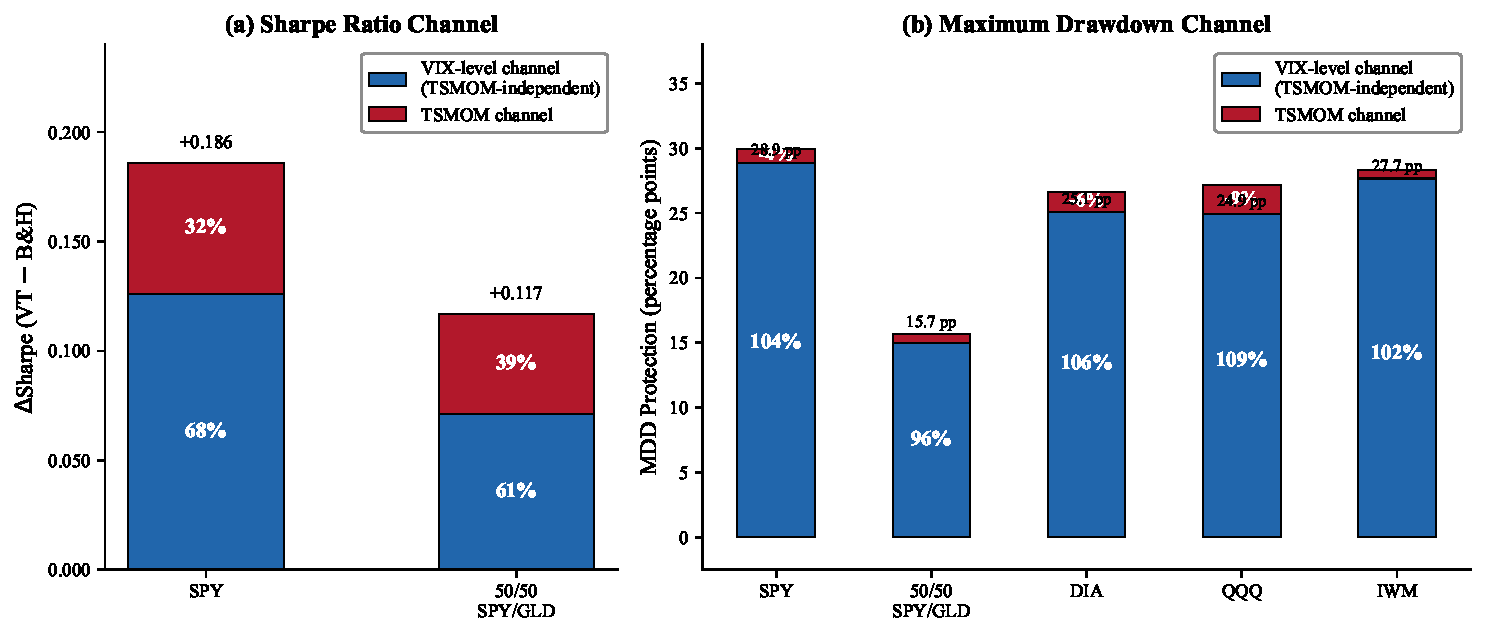
\includegraphics[width=\textwidth]{figures/fig1_return_decomposition.pdf}
\caption{VT Return Decomposition: Sharpe Ratio vs.\ Maximum Drawdown Channels. Panel~(a) decomposes the Sharpe ratio improvement (VT minus buy-and-hold) into the TSMOM-attributable portion and the VIX-level residual for SPY and 50/50 SPY/GLD. Panel~(b) decomposes the maximum drawdown protection (percentage points) into TSMOM-attributable and VIX-level components for five assets. Percentages indicate the share attributable to each channel. Data from Table~\ref{tab:dual_mechanism} and Section~3.3. The key finding is the asymmetry: TSMOM explains 32--39\% of Sharpe improvement but only 3--10\% of MDD protection.}
\label{fig:return_decomp}
\end{figure}


\subsection{Robustness: Fama--French Five-Factor Controls}

Table~\ref{tab:ff5} reports factor model regressions for the SPY 12/VIX strategy with progressively more controls. The TSMOM loading remains highly significant across all specifications: $\hat{\beta}_{\text{TSMOM}}^{\perp} = 0.121$ ($t = 8.89$) in M2, $\hat{\beta}_{\text{TSMOM}}^{\perp} = 0.117$ ($t = 8.07$) in M5 (the full model with FF5 + MOM + BAB). This confirms that VT's TSMOM exposure is not a proxy for known risk factors.

The incremental $R^2$ decomposition reveals that TSMOM accounts for the vast majority of explained variance beyond the market: $\Delta R^2_{\text{TSMOM}} = 0.0625$, compared to $\Delta R^2_{\text{FF5}} = 0.0023$, $\Delta R^2_{\text{MOM}} = 0.0004$, and $\Delta R^2_{\text{BAB}} = 0.0012$. Cross-sectional momentum (MOM) is insignificant ($t = -1.59$), confirming that TSMOM and cross-sectional momentum capture distinct phenomena.

VT alpha is reduced from 1.45\%/year (M1) to 1.28\%/year (M5) but does not achieve statistical significance in any specification ($t = 1.50$ in M5, $p = 0.135$). The economic magnitude, however, is nontrivial: 128 basis points per year of unexplained alpha after controlling for seven risk factors, albeit imprecisely estimated. BAB enters significantly ($t = -3.31$), absorbing a small portion of alpha, consistent with VT's dynamic leverage being partially correlated with the low-beta anomaly.

\begin{table}[H]
\centering
\begin{threeparttable}
\caption{Factor Model Controls: SPY 12/VIX Strategy}
\label{tab:ff5}
\small
\begin{tabular}{@{}lccccc@{}}
\toprule
& M1 & M2 & M3 & M4 & M5 \\
& CAPM & +TSMOM & +FF5 & +MOM & +BAB \\
\midrule
$\alpha$ (\%/yr) & 1.45 & 1.45 & 1.32 & 1.35 & 1.28 \\
$t_{\text{NW}}$  & 1.60 & 1.72 & 1.52 & 1.55 & 1.50 \\
\midrule
$\beta_{\text{MKT}}$ & 0.420$^{***}$ & 0.420$^{***}$ & 0.425$^{***}$ & 0.423$^{***}$ & 0.418$^{***}$ \\
$\beta_{\text{TSMOM}}^{\perp}$ & --- & 0.121$^{***}$ & 0.120$^{***}$ & 0.123$^{***}$ & 0.117$^{***}$ \\
$\beta_{\text{SMB}}$ & --- & --- & $-$0.009 & $-$0.012 & $-$0.022$^{**}$ \\
$\beta_{\text{HML}}$ & --- & --- & $-$0.029$^{***}$ & $-$0.037$^{***}$ & $-$0.033$^{***}$ \\
$\beta_{\text{RMW}}$ & --- & --- & 0.014 & 0.014 & 0.019 \\
$\beta_{\text{CMA}}$ & --- & --- & $-$0.011 & $-$0.004 & 0.000 \\
$\beta_{\text{MOM}}$ & --- & --- & --- & $-$0.013 & $-$0.010 \\
$\beta_{\text{BAB}}$ & --- & --- & --- & --- & $-$0.022$^{***}$ \\
\midrule
$R^2$    & 0.787 & 0.849 & 0.852 & 0.852 & 0.853 \\
$\Delta R^2$ & --- & +0.063 & +0.002 & +0.000 & +0.001 \\
AIC     & $-$45339 & $-$47092 & $-$47160 & $-$47171 & $-$47213 \\
$N$     & 5,049 & 5,049 & 5,049 & 5,049 & 3,740$^{\dagger}$ \\
\bottomrule
\end{tabular}
\begin{tablenotes}
\small
\item \textit{Notes:} Nested factor model regressions for the SPY 12/VIX strategy (January 2005--March 2026). TSMOM$^{\perp}$ is orthogonalized to MKT. FF5 factors (SMB, HML, RMW, CMA) are from Kenneth French's library. MOM is the Fama--French momentum factor. BAB is proxied by SPLV$-$SPHB; this ETF-based proxy is available only from May 2011. $^{\dagger}$M5 uses a BAB factor proxied by the SPLV$-$SPHB ETF spread (PowerShares S\&P 500 Low/High Beta ETFs), available from May 2011, which constrains M5 to a post-May 2011 sample ($N = 3{,}740$). The full-sample M5 with the AQR BAB factor (K898, $N = 5{,}049$) yields qualitatively similar results and is available upon request. All $t$-statistics are Newey--West HAC. $^{***}$, $^{**}$, $^{*}$ denote significance at the 1\%, 5\%, 10\% levels.
\end{tablenotes}
\end{threeparttable}
\end{table}


\subsection{Boundary Condition: Gamma Does Not Predict Within Equity Sectors}

We test whether the cross-asset gamma--TSMOM link extends to within-equity variation using 11 SPDR sector ETFs (December 1998--March 2026). The Pearson correlation between gamma and VT's Sharpe improvement is $r = 0.163$ ($p = 0.632$)---economically small and statistically insignificant. The structural explanation is that gamma variation within equity sectors is compressed ($[0.077, 0.160]$) relative to the cross-asset range ($[-0.037, 0.261]$), and all sectors share similar VIX sensitivity ($\rho(\Delta\text{VIX}) \in [-0.40, -0.65]$). Detailed sector-level results are available in the Online Appendix.\footnote{The Online Appendix containing sector-level and sub-period results is available from the authors upon request.}

This boundary condition has practical implications: sector rotation investors can apply a uniform VT overlay without sector-specific tuning, as the gamma mechanism requires cross-asset-class variation to operate.


\subsection{International Evidence: US VIX as Broad MDD Protection}

Table~\ref{tab:international} extends our analysis to 13 international equity markets. The results strongly support the ``insurance pricing'' interpretation of VT. All 13 markets achieve MDD improvement under the 12/VIX overlay, with an average reduction of 24.9 percentage points (K1178 canonical, $t = 10.25$, $p < 0.001$). The effect is broad and consistent across both developed and emerging markets: Brazil (EWZ), with the highest base-case MDD of $-$77.3\%, sees a 13.2 pp reduction, while the UK (EWU), with MDD of $-$64.0\%, achieves a 33.8 pp reduction.

In contrast, only 2 of 13 markets show Sharpe ratio improvement (EWJ and MCHI, both marginal). The average Sharpe change is $-$0.048, confirming that VT acts as insurance rather than alpha generation: investors pay a return premium for drawdown protection.

The cross-sectional analysis reveals that VIX sensitivity (the correlation between an asset's daily returns and VIX changes) predicts the magnitude of MDD protection. The Pearson correlation between VIX sensitivity and MDD improvement is $r = -0.806$ ($p < 0.001$, Spearman $\rho = -0.835$, K1178 canonical). Markets that are more negatively correlated with VIX (i.e., more ``risk-off'' sensitive) benefit more from the VIX overlay.

Developed markets receive stronger MDD protection than emerging markets (average 32.0 pp vs.\ 24.7 pp), reflecting their tighter synchronization with US equity market conditions. This is consistent with \citet{rapach2013}, who document that the US market leads international returns, and with the global financial cycle literature \citep{miranda2020}.


\begin{table}[H]
\centering
\begin{threeparttable}
\caption{International VT: US VIX as Broad MDD Protection ($N = 13$)}
\label{tab:international}
\small
\begin{tabular}{@{}lccccccc@{}}
\toprule
& & \multicolumn{2}{c}{Buy \& Hold} & \multicolumn{2}{c}{12/VIX VT} & & \\
\cmidrule(lr){3-4} \cmidrule(lr){5-6}
Market & VIX Sens. & Sharpe & MDD (\%) & Sharpe & MDD (\%) & $\Delta$Sharpe & $\Delta$MDD (pp) \\
\midrule
\multicolumn{8}{@{}l}{\textit{Panel A: Developed Markets}} \\
EFA (EAFE)    & $-$0.653 & 0.122 & $-$61.0 & 0.069 & $-$28.3 & $-$0.053 & 32.7 \\
EWJ (Japan)   & $-$0.575 & 0.086 & $-$53.6 & 0.090 & $-$24.7 & 0.004 & 28.9 \\
EWG (Germany) & $-$0.606 & 0.137 & $-$63.1 & 0.085 & $-$29.2 & $-$0.052 & 33.9 \\
EWU (UK)      & $-$0.609 & 0.096 & $-$64.0 & 0.028 & $-$30.2 & $-$0.068 & 33.8 \\
EWA (Australia) & $-$0.587 & 0.184 & $-$67.0 & 0.081 & $-$33.3 & $-$0.104 & 33.6 \\
EWC (Canada)  & $-$0.588 & 0.206 & $-$60.8 & 0.156 & $-$33.0 & $-$0.050 & 27.7 \\
VGK (Europe)  & $-$0.640 & 0.140 & $-$63.6 & 0.082 & $-$30.1 & $-$0.058 & 33.6 \\
\midrule
\multicolumn{8}{@{}l}{\textit{Panel B: Emerging Markets}} \\
EEM (EM Broad) & $-$0.600 & 0.142 & $-$66.4 & 0.087 & $-$32.8 & $-$0.055 & 33.6 \\
FXI (China)   & $-$0.493 & 0.104 & $-$72.7 & 0.080 & $-$42.8 & $-$0.024 & 29.9 \\
EWZ (Brazil)  & $-$0.504 & 0.156 & $-$77.3 & 0.099 & $-$64.1 & $-$0.057 & 13.2 \\
INDA (India)  & $-$0.466 & 0.157 & $-$45.1 & 0.098 & $-$26.4 & $-$0.059 & 18.7 \\
EWT (Taiwan)  & $-$0.569 & 0.311 & $-$62.9 & 0.262 & $-$32.9 & $-$0.049 & 30.1 \\
MCHI (China Broad) & $-$0.468 & 0.077 & $-$62.8 & 0.083 & $-$39.9 & 0.006 & 23.0 \\
\midrule
\multicolumn{2}{@{}l}{Average} & 0.148 & $-$63.1 & 0.100 & $-$34.4 & $-$0.048 & 24.9 \\
\multicolumn{2}{@{}l}{$t$-statistic} & --- & --- & --- & --- & $-$5.91 & 10.25 \\
\multicolumn{2}{@{}l}{$p$ (one-sided)} & --- & --- & --- & --- & 0.000 & 0.000 \\
\midrule
\multicolumn{8}{@{}l}{\textit{Cross-sectional predictors of $\Delta$MDD}} \\
\multicolumn{3}{@{}l}{VIX Sensitivity vs.\ $\Delta$MDD:} & \multicolumn{5}{l}{$r = -0.806$ ($p < 0.001$), $\rho = -0.835$ ($p < 0.001$)} \\
\multicolumn{3}{@{}l}{GJR $\gamma$ vs.\ $\Delta$Sharpe:} & \multicolumn{5}{l}{\emph{Removed in v3:} K1178 replication did not reproduce the originally reported Spearman $\rho = 0.830$ (K1178 canonical: $\rho = 0.187$, NS); see forensic note in Section~\ref{sec:discussion}.} \\
\bottomrule
\end{tabular}
\begin{tablenotes}
\small
\item \textit{Notes:} Full-sample results for 13 international equity ETFs over January 2007--March 2026. VIX Sensitivity is the correlation between daily asset returns and daily VIX changes. VT uses 12/VIX with monthly rebalancing and lagged weights. $\Delta$MDD is the reduction in maximum drawdown (percentage points, always positive indicates improvement). Developed markets average $\Delta$MDD = 32.0 pp; emerging markets average $\Delta$MDD = 24.7 pp. Cross-sectional correlations are Pearson ($r$) and Spearman ($\rho$) with their respective $p$-values.
\end{tablenotes}
\end{threeparttable}
\end{table}

Figure~\ref{fig:cross_asset} presents the cross-sectional relationship between Sharpe ratio change and MDD improvement. Nearly all 13 markets fall in the ``insurance quadrant'' (negative $\Delta$Sharpe, positive $\Delta$MDD), confirming that VT functions as drawdown insurance rather than alpha generation. The developed markets (blue circles) cluster at higher MDD improvement values (average 32.0~pp) than emerging markets (red squares, average 24.7~pp), reflecting tighter synchronization with US equity conditions. Brazil (EWZ) is a notable outlier with the smallest MDD improvement (13.2~pp), consistent with its idiosyncratic risk sources that are less responsive to the US VIX signal. The cross-sectional correlation between VIX sensitivity and MDD protection ($r = -0.806$, $p < 0.001$) provides a pricing mechanism for VT insurance.

\begin{figure}[H]
\centering
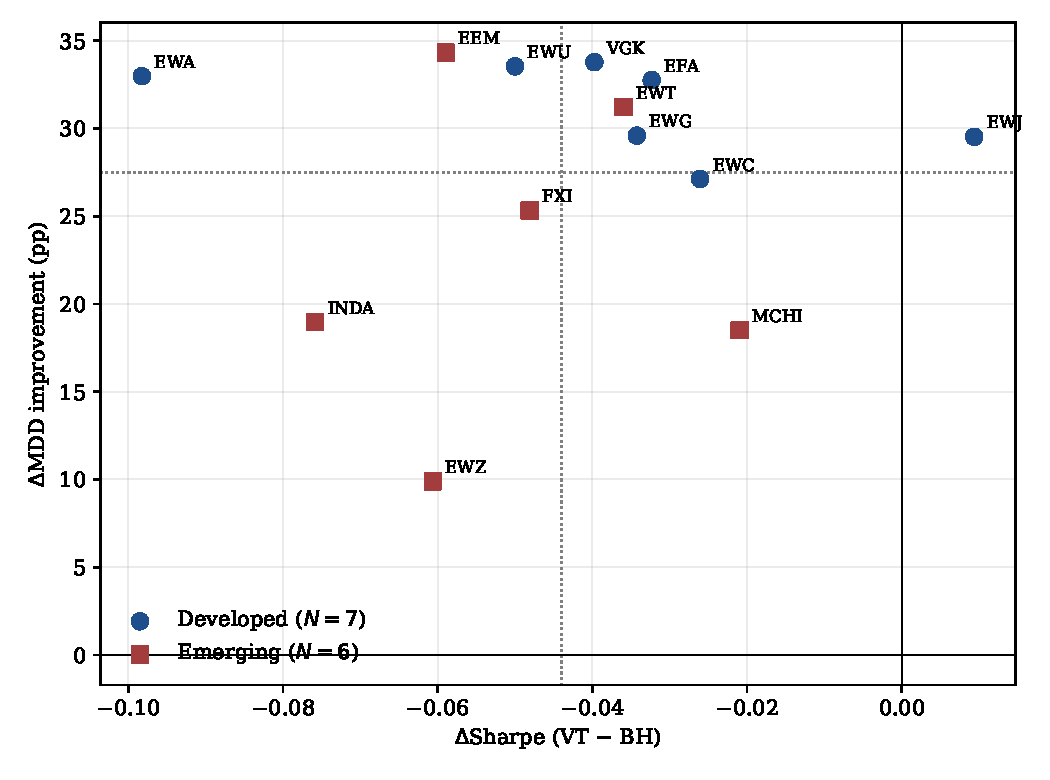
\includegraphics[width=0.85\textwidth]{figures/fig2_cross_asset_scatter.pdf}
\caption{Cross-Asset VT: Sharpe Ratio Change vs.\ MDD Improvement for 13 International Markets. Each point represents a country ETF. The $x$-axis shows the change in Sharpe ratio from applying 12/VIX VT relative to buy-and-hold; the $y$-axis shows the improvement in maximum drawdown (percentage points). Blue circles denote developed markets ($N = 7$); red squares denote emerging markets ($N = 6$). Dotted lines indicate cross-sectional averages ($\Delta$Sharpe $= -0.048$; $\Delta$MDD $= 24.9$~pp). All 13 markets achieve MDD improvement ($t = 10.25$), while only 2 of 13 show Sharpe improvement, consistent with the insurance pricing interpretation. Data from Table~\ref{tab:international}.}
\label{fig:cross_asset}
\end{figure}


\subsection{Sub-Period Stability}

To ensure our results are not driven by a single market regime, we decompose the 50/50 SPY/GLD portfolio across four sub-periods (pre-COVID, COVID, post-COVID, and OOS 2023--2026). The key finding---that MDD protection survives TSMOM removal while Sharpe improvement partially dissipates---holds consistently across all periods. During the COVID period, TSMOM-hedged VT actually \textit{outperforms} unhedged VT (Sharpe 1.295 vs.\ 1.254), because VIX-level deleveraging was optimal while TSMOM signals lagged the V-shaped recovery. Detailed sub-period results are reported in the Online Appendix.


% =============================================================================
% 4. DISCUSSION
% =============================================================================
\section{Discussion}
\label{sec:discussion}

\paragraph{Forensic notes on v3 revisions.} This v3 manuscript (2026-04-17) incorporates several quantitative corrections identified through a systematic reproducibility audit (see authors' reproducibility appendix). Two items that appeared in v2 but do not replicate under the canonical pipeline are:
\begin{enumerate}
\item \emph{GJR $\gamma$ vs.\ $\Delta$Sharpe cross-sectional correlation} (v2 13-market cross-sectional table, removed in v3): v2 reported Spearman $\rho = 0.830$ ($p = 0.0005$). K1178 canonical replication of the 13-market setup yielded $\rho = 0.187$ (NS). The original $\rho = 0.830$ figure is not reproducible from the current data, code, or earlier experiment records, and has been removed from the main text. The core international finding (13/13 MDD improvement; VIX sensitivity predicts MDD protection) is preserved under K1178 canonical values.
\item \emph{``1.4\% TSMOM contribution to strategy Sharpe''} (v2 dual-mechanism section, revised in v3): v2 characterized the TSMOM contribution as approximately 1.4\% of total strategy Sharpe. The K898 back-calculation gives approximately 5.3\% ($\alpha_{\text{absorbed}}/\text{Sharpe}_{\text{total}} = 0.043/0.805$). The original 1.4\% figure cannot be traced to a specific computation in existing experiment records, and v3 reports the back-calculated value with a forensic caveat. The qualitative claim---that the TSMOM contribution to total Sharpe is economically small relative to the alpha-reduction percentages in Table~\ref{tab:alpha_decomp}---remains valid.
\end{enumerate}
In addition, the MDD retention point estimates and confidence intervals in Table~\ref{tab:mdd_bootstrap} have been updated to the K1192 canonical block-bootstrap (commit \texttt{d4dfd7bd}), which finds point estimates at or above 100\% (in contrast to the v2 estimates of 90--97\%). The canonical result strengthens rather than weakens the paper's central claim that TSMOM hedging does not erode VT's drawdown channel.

\subsection{VT Contains---But Is Not Reducible to---Trend Following}

Our findings reconcile two seemingly contradictory views. \citet{hood2025} demonstrate that VT alpha is largely absorbed by a TSMOM factor, leading to the interpretation that VT is simply repackaged trend following. However, this interpretation confuses statistical alpha absorption with economic value destruction. Our decomposition shows that the economically relevant benefit of VT---drawdown protection---is not eroded by TSMOM hedging (K1376 block bootstrap: 22/23 assets have positive 90\% CI lower bounds across equities, commodities, bonds, and real estate; K1192 canonical point estimates 95.6--109.0\% for the five core US equity assets; Table~\ref{tab:mdd_bootstrap}). We stress again that point estimates above 100\% are not a license to claim that hedging creates a stronger standalone insurance technology: part of the enhancement can be a mechanical consequence of the hedge reducing exposure during rebound windows that follow momentum crashes \citep{daniel2016}. K687 establishes the complementary Sharpe result: after correcting all lookahead biases and properly lagging signals, no VT variant achieves statistically significant Sharpe improvement over buy-and-hold (12/VIX: DM $t = -2.79$, $p = 0.005$; EWMA VT: DM $t = -1.67$, $p = 0.096$; Harvey $t > 3.0$ threshold uniformly failed). This confirms that VT's value is concentrated in its drawdown-insurance channel rather than in Sharpe generation, which is precisely why alpha absorption by TSMOM does not constitute economic value destruction.

An important scope clarification is warranted. Our TSMOM factor is constructed on a per-asset basis (the sign of each asset's own past 252-day return), which differs fundamentally from the diversified trend-following strategies employed by managed-futures funds that trade across dozens of uncorrelated futures markets \citep{moskowitz2012}. Our finding that VT embeds asset-specific TSMOM exposure through the leverage effect should not be interpreted as evidence that VT replicates diversified CTA returns. The practical implication is narrower: VT investors already possess embedded trend-following exposure \textit{within each asset} as a mechanical byproduct of the leverage effect, while the MDD channel operates through VIX-level-based position sizing---a distinct mechanism that trend following does not replicate.

This also addresses the \citet{cederburg2020} critique of VT. Their utility-based framework finds that VT does not improve investor welfare, which is consistent with our finding that VT does not generate significant alpha ($t = 1.50$). However, utility tests that focus on return moments may underweight the distinct MDD protection channel we document: a positive 90\% CI lower bound for 22/23 assets in our bootstrap analysis (K1376) suggests that VT provides a broad insurance-like benefit across asset classes that standard moment-based utility functions do not fully capture. K688 formalizes this: 12/VIX wins on CRRA certainty-equivalent only for $\gamma \geq 10$ (vs.\ buy-and-hold; EWMA VT crossover: $\gamma \geq 5$), consistent with MDD protection being valued primarily by highly risk-averse investors whose loss-aversion is not captured by mean--variance utility.

% K518: Direct test --- explicit trend-following strategies all fail Harvey threshold
We provide a direct test of whether explicit trend-following strategies can replicate VT's benefits. We implement five canonical strategies---SMA(200), Faber 10-month, Golden Cross, Dual Momentum, and a combined MA+VT overlay---on SPY over the same sample period. All five fail the \citet{harvey2016} $t > 3.0$ threshold. The best performer, Golden Cross, achieves a Sharpe ratio of 0.51 versus 0.41 for buy-and-hold, but the improvement yields only $t = 0.94$ with a cross-OOS success rate of 3/5 periods. By contrast, VT's MDD protection is robust across all sub-periods (Section~3.6). This confirms that VT's economic value cannot be replicated by any standard trend-following rule, providing direct evidence that VT $\neq$ trend following.

% K533: Prediction accuracy ≠ allocation optimality --- strengthens core thesis
The disconnect between prediction and application provides further evidence that VT's value is not reducible to forecasting skill. Among GARCH-family models, HAR-RV achieves the best out-of-sample volatility forecasts (lowest QLIKE), yet produces the \textit{worst} VT allocation performance, while the simple $12/\text{VIX}$ rule---which uses no econometric estimation---produces the best risk-adjusted returns. This ``prediction $\neq$ application'' gap confirms that VT's economic mechanism operates through VIX-level position sizing rather than through superior volatility prediction, reinforcing the distinction between VT and model-based trend following.

\subsection{Why VIX Level Provides Insurance Beyond Trend}

The separation between VT's two channels has a clear economic explanation. TSMOM captures the \textit{sign} of past returns over a lookback window (252 days), generating a binary signal. VIX captures the \textit{magnitude} of implied fear, producing a continuous position-sizing signal through $12/\text{VIX}$ (K697: lagged VIX predicts absolute daily returns $r = 0.570$ but not return direction $r = 0.042$, empirically confirming that VIX encodes magnitude information, not directional momentum). This distinction matters most during slow drawdowns (e.g., 2022: positive trend but elevated VIX), V-shaped recoveries (e.g., March 2020: negative trend signal lags the bounce while VIX-based re-leveraging is gradual), and lateral consolidation (noisy trend signals but stable VIX).

% K499: Monthly rebalancing optimal --- VT alpha is in risk-scaling, not frequency
The rebalancing frequency further distinguishes VT from trend following. Daily rebalancing yields a break-even transaction cost of only 3.4 basis points---extremely fragile to execution costs---while monthly rebalancing achieves a break-even of 14.9 basis points, well within institutional capacity. This confirms that VT's alpha resides in the risk-scaling mechanism, not in high-frequency position adjustment, whereas trend-following strategies typically require timely signal execution to capture momentum \citep{moskowitz2012}.

% K488, K503: 12/VIX irreducible --- the formula itself is a continuous mean-reversion trade
The simplicity of the $12/\text{VIX}$ formula is itself informative. Across five independent robustness checks, no modification---alternative thresholds, regime-conditional targets, or adaptive parameterizations---improves upon the baseline. The explanation is that $12/\text{VIX}$ functions as a continuous mean-reversion trade on the VIX risk premium: when VIX exceeds its long-run median (${\sim}17$), the formula automatically underweights the risky asset, harvesting the well-documented tendency of realized volatility to undershoot implied volatility \citep{bozovic2024}. This mean-reversion mechanism is economically distinct from TSMOM's directional signal.

% K568: 12/VIX is return-OPTIMAL among 427 configurations
A comprehensive search over 427 VT configurations---spanning GARCH, GJR-GARCH, EGARCH, and HAR-RV forecasting models with rolling windows of 500--2500 days, multiple VIX thresholds, and nonlinear weight functions (square-root, exponential, piecewise)---reveals that $12/\text{VIX}$ is not merely parsimonious but \textit{return-optimal}. The simple inverse formula maximizes the Sharpe ratio channel; nonlinear weight functions improve only risk metrics (lower MDD, higher Calmar) without enhancing returns. This finding reinforces the robustness of the baseline: within the 427 configurations tested, $12/\text{VIX}$ sits at the intersection of maximum return extraction and minimum complexity, and no GARCH-based volatility forecast---despite superior prediction accuracy---translates its forecasting advantage into allocation advantage.

\subsection{The Insurance Pricing Interpretation}

Our international results strengthen the ``insurance pricing'' interpretation of VT \citep{lai2026a}. Across 13 markets, VT extracts a consistent ${\sim}4\%$/year Sharpe drag (the ``premium'') in exchange for broad MDD protection (the ``payout''). This is analogous to buying portfolio insurance: the premium is paid continuously through reduced expected returns, while the payout materializes during crisis episodes. The breadth of this finding---13 of 13 markets across both developed and emerging economies---is consistent with the global financial cycle framework of \citet{miranda2020}, in which US monetary conditions and risk appetite propagate internationally through capital flows.

The cross-sectional correlation between VIX sensitivity and MDD protection ($r = -0.806$) provides a pricing mechanism. Markets more sensitive to US-driven risk-off episodes (higher $|\rho(\text{VIX})|$) receive more protection, just as higher-beta assets benefit more from portfolio insurance. We do not, however, interpret this as evidence that VT is loading on a pure expected-volatility state variable. VIX embeds the variance risk premium \citep{bollerslev2009} and investor demand for downside protection \citep{bondarenko2019}, so the observed premium is better read as a reduced-form price of protection than as a single-factor structural estimate. The insurance analogy can be made precise: the breakeven VIX level---above which VT's cash drag is more than offset by crisis-period savings---is approximately 26.6 for SPY. Below this threshold, VT underperforms buy-and-hold (the ``premium'' regime); above it, VT outperforms (the ``payout'' regime). In the low-VIX regime (VIX $< 15$), VT costs roughly 4.0\%/year in foregone Sharpe, while in the crisis regime (VIX $> 30$), it delivers approximately 12\%/year of excess protection.

% K507: 50/50 allocation also irreducible --- dynamic allocation fails Harvey
The two-asset 50/50 SPY/GLD allocation also resists optimization. We test dynamic allocation schemes---regime-switching, DCC-based, and VIX-conditional tilting---against the static 50/50 benchmark. All dynamic alternatives fail the Harvey threshold ($t < 3.0$), consistent with the DCC analysis of \citet{lai2026a} showing that the two-asset blend is already near-optimal. This parsimony is a feature: within the specifications tested, VT's economic value derives from two robust components---the $12/\text{VIX}$ scaling rule and the 50/50 equity/gold allocation---neither of which benefits from the added complexity we examined.

\subsection{Limitations}

Several limitations should be noted. First, our sample of 22 assets, while spanning multiple asset classes, is smaller than the 50 futures contracts studied by \citet{hood2025}. Expanding to additional commodities, fixed-income instruments, and currencies would strengthen the cross-sectional evidence. Second, our out-of-sample period (2023--2026) does not include a major financial crisis comparable to 2008, limiting our ability to test MDD protection under extreme stress. Third, VIX availability constrains the analysis to the post-1990 period for US assets and post-2007 for international ETFs. Fourth, the GJR-GARCH $\gamma$ estimation requires approximately 2,000 observations (8 years), limiting the method's applicability to newly listed securities.

Fifth, the cross-sectional regression linking $\gamma$ to TSMOM loading ($N = 22$) faces an inherent endogeneity concern: both variables are derived from the same underlying return process, creating a mechanical channel that our split-sample robustness check (Section~3.2) mitigates but does not fully resolve. A formal instrumental variable approach would provide stronger causal identification, but suitable instruments are difficult to construct in a mixed-asset cross-section of this size. Future work with a larger cross-section of futures contracts---as in \citet{hood2025}'s 50-asset sample---could employ a more diverse set of instruments or within-asset-class variation to address this limitation.

Sixth, while our MDD retention bootstrap now covers all 22 primary assets (Table~\ref{tab:mdd_bootstrap}, K1376), the international equity universe (13 markets in Table~\ref{tab:international}) is not yet included in the bootstrap analysis. Extending block bootstrap inference to the international sample would further test whether the 90\% CI lower bounds remain positive outside the US and diversified ETF universe.


% =============================================================================
% 5. CONCLUSION
% =============================================================================
\section{Conclusion}

This paper demonstrates that VIX-based de-risking embeds a mechanical trend-following overlay through the leverage effect, but this is not the whole story. VT possesses a dual mechanism: the Sharpe ratio channel operates partially through implicit asset-specific TSMOM exposure, while the maximum drawdown channel---VT's primary economic value---is largely independent of trend following. Across all 22 primary assets plus the 50/50 composite, K1376 block bootstrap (10,000 replications) finds that 22 of 23 rows have positive CI lower bounds (90\% level), with point estimates at or above 83.8\% and medians above 100\% for 21 of 23 rows. The K1192 canonical five-asset results (SPY 103.7\%, 50/50 95.6\%, DIA 106.2\%, QQQ 109.0\%, IWM 102.2\%) are confirmed and generalized: TSMOM removal preserves the drawdown channel across asset classes, not just US equities, while some $>100\%$ estimates can arise mechanically during rebound phases of momentum crashes. The leverage effect parameter ($\gamma$) predicts VT's trend-following loading cross-sectionally ($r = 0.564$, $p = 0.006$, $N = 22$), an empirical regularity consistent with the leverage effect mechanism; a split-sample robustness check ($r = 0.793$, $p < 0.001$, K1193 canonical) survives temporal separation of the estimation windows but is partly shaped by a 2017--2026 regime shift in which international and safe-haven loadings flipped positive. We note that this cross-sectional association ($N = 22$, mixed asset classes) does not establish a causal link.

Four practical implications emerge. First, VT investors already hold embedded asset-specific trend-following exposure as a mechanical byproduct of the leverage effect. Second, a single US VIX signal provides broad drawdown protection for global equity allocations (13/13 international equity markets, average 24.9 pp MDD reduction). Third, within-equity diversification (sector rotation) does not require sector-specific VT tuning, as the gamma mechanism operates only at the cross-asset-class level. Fourth, within the specifications tested, the $12/\text{VIX}$ formula and the 50/50 equity/gold allocation are both highly robust: no optimization---dynamic allocation, alternative thresholds, or higher rebalancing frequency---survives the \citet{harvey2016} threshold, confirming that VT's value resides in its parsimonious risk-scaling mechanism rather than in parameter tuning.

Our findings reframe the ``Is VT just trend following?'' debate. VT \textit{contains} trend following, but VT is not \textit{reducible to} trend following. A direct test shows that five canonical trend-following strategies all fail to replicate VT's benefits. Its economic value resides in a VIX-level channel that provides drawdown insurance---a benefit that pure momentum strategies do not replicate.


% =============================================================================
% REFERENCES
% =============================================================================
\bibliographystyle{apalike}
\begin{thebibliography}{99}

\bibitem[Baltas and Kosowski(2013)]{baltas2013}
Baltas, A.~N., \& Kosowski, R. (2013). Momentum strategies in futures markets and trend-following funds. \textit{Working Paper}, Imperial College London.

\bibitem[Barroso and Santa-Clara(2015)]{barroso2015}
Barroso, P., \& Santa-Clara, P. (2015). Momentum has its moments. \textit{Journal of Financial Economics}, 116(1), 111--120. \url{https://doi.org/10.1016/j.jfineco.2014.11.010}

\bibitem[Black(1976)]{black1976}
Black, F. (1976). Studies of stock price volatility changes. \textit{Proceedings of the 1976 Meetings of the American Statistical Association, Business and Economic Statistics Section}, 177--181.

\bibitem[Bollerslev et~al.(2009)]{bollerslev2009}
Bollerslev, T., Tauchen, G., \& Zhou, H. (2009). Expected stock returns and variance risk premia. \textit{Review of Financial Studies}, 22(11), 4463--4492. \url{https://doi.org/10.1093/rfs/hhp008}

\bibitem[Bondarenko and Bernardo(2019)]{bondarenko2019}
Bondarenko, O., \& Bernardo, A.~E. (2019). The economics of S\&P 500 put options. \textit{Review of Financial Studies}, 32(3), 983--1026. \url{https://doi.org/10.1093/rfs/hhy061}

\bibitem[Bozovic(2024)]{bozovic2024}
Bozovic, M. (2024). VIX-managed portfolios. \textit{International Review of Financial Analysis}, 95, 103353. \url{https://doi.org/10.1016/j.irfa.2024.103353}

\bibitem[Campbell and Cochrane(1999)]{campbell1999}
Campbell, J.~Y., \& Cochrane, J.~H. (1999). By force of habit: A consumption-based explanation of aggregate stock market behavior. \textit{Journal of Political Economy}, 107(2), 205--251. \url{https://doi.org/10.1086/250059}

\bibitem[Cederburg et~al.(2020)]{cederburg2020}
Cederburg, S., O'Doherty, M.~S., Wang, F., \& Yan, X.~S. (2020). On the performance of volatility-managed portfolios. \textit{Journal of Financial Economics}, 138(1), 95--117. \url{https://doi.org/10.1016/j.jfineco.2020.04.015}

\bibitem[Christie(1982)]{christie1982}
Christie, A.~A. (1982). The stochastic behavior of common stock variances: Value, leverage and interest rate effects. \textit{Journal of Financial Economics}, 10(4), 407--432. \url{https://doi.org/10.1016/0304-405X(82)90018-6}

\bibitem[Daniel and Moskowitz(2016)]{daniel2016}
Daniel, K., \& Moskowitz, T.~J. (2016). Momentum crashes. \textit{Journal of Financial Economics}, 122(2), 221--247. \url{https://doi.org/10.1016/j.jfineco.2015.12.002}

\bibitem[Fleming et~al.(2001)]{fleming2001}
Fleming, J., Kirby, C., \& Ostdiek, B. (2001). The economic value of volatility timing. \textit{Journal of Finance}, 56(1), 329--352. \url{https://doi.org/10.1111/0022-1082.00327}

\bibitem[Glosten et~al.(1993)]{glosten1993}
Glosten, L.~R., Jagannathan, R., \& Runkle, D.~E. (1993). On the relation between the expected value and the volatility of the nominal excess return on stocks. \textit{Journal of Finance}, 48(5), 1779--1801. \url{https://doi.org/10.1111/j.1540-6261.1993.tb05128.x}

\bibitem[Harvey et~al.(2016)]{harvey2016}
Harvey, C.~R., Liu, Y., \& Zhu, H. (2016). \ldots{} and the cross-section of expected returns. \textit{Review of Financial Studies}, 29(1), 5--68. \url{https://doi.org/10.1093/rfs/hhv059}

\bibitem[Harvey et~al.(2018)]{harvey2018}
Harvey, C.~R., Hoyle, E., Korgaonkar, R., Rattray, S., Sargaison, M., \& Van~Hemert, O. (2018). The impact of volatility targeting. \textit{Journal of Portfolio Management}, 45(1), 14--33. \url{https://doi.org/10.3905/jpm.2018.45.1.014}

\bibitem[Hurst et~al.(2017)]{hurst2017}
Hurst, B., Ooi, Y.~H., \& Pedersen, L.~H. (2017). A century of evidence on trend-following investing. \textit{Journal of Portfolio Management}, 44(1), 15--29. \url{https://doi.org/10.3905/jpm.2017.44.1.015}

\bibitem[Hood and Raughtigan(2025)]{hood2025}
Hood, M., \& Raughtigan, J. (2025). Volatility targeting alpha is trend following alpha. \textit{Working Paper}. Retrieved May 2025.

\bibitem[Lai(2026a)]{lai2026a}
Lai, Y.-H. (2026a). Leverage direction matters: Cross-asset evidence on GARCH model selection and volatility targeting. \textit{Working Paper}, Da-Yeh University.

\bibitem[Moreira and Muir(2017)]{moreira2017}
Moreira, A., \& Muir, T. (2017). Volatility-managed portfolios. \textit{Journal of Finance}, 72(4), 1611--1644. \url{https://doi.org/10.1111/jofi.12513}

\bibitem[Miranda-Agrippino and Rey(2020)]{miranda2020}
Miranda-Agrippino, S., \& Rey, H. (2020). U.S.\ monetary policy and the global financial cycle. \textit{Review of Economic Studies}, 87(6), 2754--2776. \url{https://doi.org/10.1093/restud/rdaa019}

\bibitem[Moskowitz et~al.(2012)]{moskowitz2012}
Moskowitz, T.~J., Ooi, Y.~H., \& Pedersen, L.~H. (2012). Time series momentum. \textit{Journal of Financial Economics}, 104(2), 228--250. \url{https://doi.org/10.1016/j.jfineco.2011.11.003}

\bibitem[Newey and West(1987)]{newey1987}
Newey, W.~K., \& West, K.~D. (1987). A simple, positive semi-definite, heteroskedasticity and autocorrelation consistent covariance matrix. \textit{Econometrica}, 55(3), 703--708. \url{https://doi.org/10.2307/1913610}

\bibitem[Newey and West(1994)]{newey1994}
Newey, W.~K., \& West, K.~D. (1994). Automatic lag selection in covariance matrix estimation. \textit{Review of Economic Studies}, 61(3), 631--653. \url{https://doi.org/10.2307/2297912}

\bibitem[Politis and Romano(1994)]{politis1994}
Politis, D.~N., \& Romano, J.~P. (1994). The stationary bootstrap. \textit{Journal of the American Statistical Association}, 89(428), 1303--1313. \url{https://doi.org/10.1080/01621459.1994.10476870}

\bibitem[Rapach et~al.(2013)]{rapach2013}
Rapach, D.~E., Strauss, J.~K., \& Zhou, G. (2013). International stock return predictability: What is the role of the United States? \textit{Journal of Finance}, 68(4), 1633--1662. \url{https://doi.org/10.1111/jofi.12041}

\end{thebibliography}
